\documentclass[12pt,a4paper,onecolumn]{article}

% Packages
\usepackage{lipsum}
\usepackage{xcolor}
\usepackage{graphicx}
\usepackage{amsmath}
\usepackage[colorlinks=true,linkcolor=black,urlcolor=blue,citecolor=black]{hyperref}
\usepackage{listings}
\usepackage{tikz}
\usepackage{pgfplots}
\usepackage{array}
\usepackage{booktabs}
\usepackage{float}

% Defined colors
\definecolor{customgreen}{RGB}{45, 135, 48}
\definecolor{codeblue}{RGB}{0, 102, 204}
\definecolor{codegray}{RGB}{128, 128, 128}

% Defined custom commands
\newcommand{\done}{\textbf{\color{customgreen} Done}}
\newcommand{\todo}{\textbf{\color{red} Todo}}
\newcommand{\fref}[1]{Figure~\ref{#1}}
\newcommand{\tref}[1]{Table~\ref{#1}}
\newcommand{\eref}[1]{(\ref{#1})}

% Code styling
\lstset{
    basicstyle=\ttfamily\small,
    commentstyle=\color{codegray},
    keywordstyle=\color{codeblue},
    stringstyle=\color{red},
    breakatwhitespace=false,
    breaklines=true,
    captionpos=b,
    keepspaces=true,
    numbers=left,
    numbersep=5pt,
    showspaces=false,
    showstringspaces=false,
    showtabs=false,
    tabsize=2
}

\title{Book Worm: A RAG Implementation}
\author{Julian Rosas \\\\ DSC 599: Data Science Capstone}
\date{December 11, 2025}

\begin{document}

\maketitle

\tableofcontents
\pagebreak

\begin{abstract}
This report presents Book Worm, a Retrieval-Augmented Generation (RAG) system designed specifically for multi-series books with guard rails for spoiler prevention. The app utilizes the Fandom MediaWiki API to extract and process content from multiple book series, utilizes text chunking algorithms, stores data in a ChromaDB vector database for semantic search, and uses Ollama 3.2 for answer generation. The app is used by the user providing a book series filter (optional), providing a question, the vector database is queried based on semantic retrieval, then the chunks are input to Ollama to generate and provide answers. The current implementation offers a Streamlit deployable user interface and offers easy additions for new book series for further information expansion. Future additions will include spoiler tags for chunks that include major spoilers. The book series successfully processed so far include the Red Rising and Harry Potter series with 853 total text chunks, achieving effective semantic retrieval while maintaining spoiler-free user experiences based on reading progress.
\end{abstract}

\pagebreak

\section{Introduction}

    Long-running book series create issues with having to remember so many characters or events that are re-introduced as the series progresses. Often, one might forget a certain character and what kind of impact they have had on the story thus far. Current solutions call for just looking up the character to read a quick description on their background and influence on the story so far, but this often include spoilers for major plot point including the worst kind of spoilers, deaths. These spoilers can simply come in the form of suggested searches right underneath a completely separate specific question you may have asked. 

This work introduces Book-Worm, a specialized RAG system that addresses these challenges through several key contributions:

\begin{enumerate}
\item \textbf{Multi-Series Architecture}: A modifiable configuration system supporting multiple book series with different structures
\item \textbf{Smart Chunking}: Efficient text segmentation algorithms optimized for narrative content
\item \textbf{Automated Data Pipeline}: End-to-end processing from wiki sources to query-able vector embeddings
\item \textbf{Context-Aware LLM Integration}: LLM response generation that synthesizes retrieved information while respecting spoiler constraints and reading progress
\item \textbf{Streamlit Deployment}: Deployment through Streamlit to provide an easy-to-use interface
\end{enumerate}

The current implementation demonstrates practical applicability using long-running series including Red Rising by Pierce Brown and Harry Potter by J.K. Rowling, with  support for easy additions for other series.

\section{Related Work}

\subsection{Book QA: Stories of Challenges and Opportunities}
Angelidis et al. (2019) introduced BookQA, a question-answering research system that implemented AI models to answer questions given a full book. It uses a retrieval and reasoning pipeline. The retriever finds passages in a book that are most relevant to a question (using Bert-based embedding models). Then a memory network is used to read the passages and perform multi-hop reasoning to infer an answer. The implementation was tested on the NarrativeQA dataset. Book Worm differs from this work through a retrieval-augmented generation implementation where you can set up a library of multiple books from different series through the Fandom API. The RAG implementation allows for spoiler-aware answers generated by an LLM vs the BookQA implementation that focuses on retrievals for one specific query. Book Worm offers more open-ended queries with constraints to limit spoiling.

\subsection{Frustratingly Hard Evidence Retrieval for QA Over Books}
Mou et al. (2020) further worked n book QA by presenting a system that tackles the challenge of QA over full-length books. It worked by receiving a question over a long book, then the system retrieves supporting evidence over the book and generates an answer. They experimented with BERT or GPT-2 for retrieval and reading but struggled with evidence retrieval, especially given long sources like an entire book. Even when increasing the number of passages retrieved, the model did not always perform better. This is very similar to my approach, but I am again using the Fandom API so questions might be more limited. But Book Worm is meant for general overviews to assist readers as they are progressing through a story rather than specific answers. This also allows for less data processing, but also makes it more difficult to ensure an answer is being answered correctly if it does become specific. 

\section{Proposed Approach}

\subsection{Data Extraction and Processing}

The system utilizes the Fandom MediaWiki API to extract structured content from series-specific wikis. The extraction process involves:

\begin{enumerate}
\item \textbf{API Configuration}: Series-specific wiki endpoints and page titles
\item \textbf{WikiText Parsing}: Conversion of MediaWiki markup to clean text
\item \textbf{Section Extraction}: Hierarchical content organization by page sections
\item \textbf{Metadata}: Addition of series, book number, and character information
\end{enumerate}

\subsection{System Architecture Overview}

The Book-Worm system follows a comprehensive RAG architecture as illustrated in \fref{fig:system_architecture}:

\begin{figure}[h]
\centering
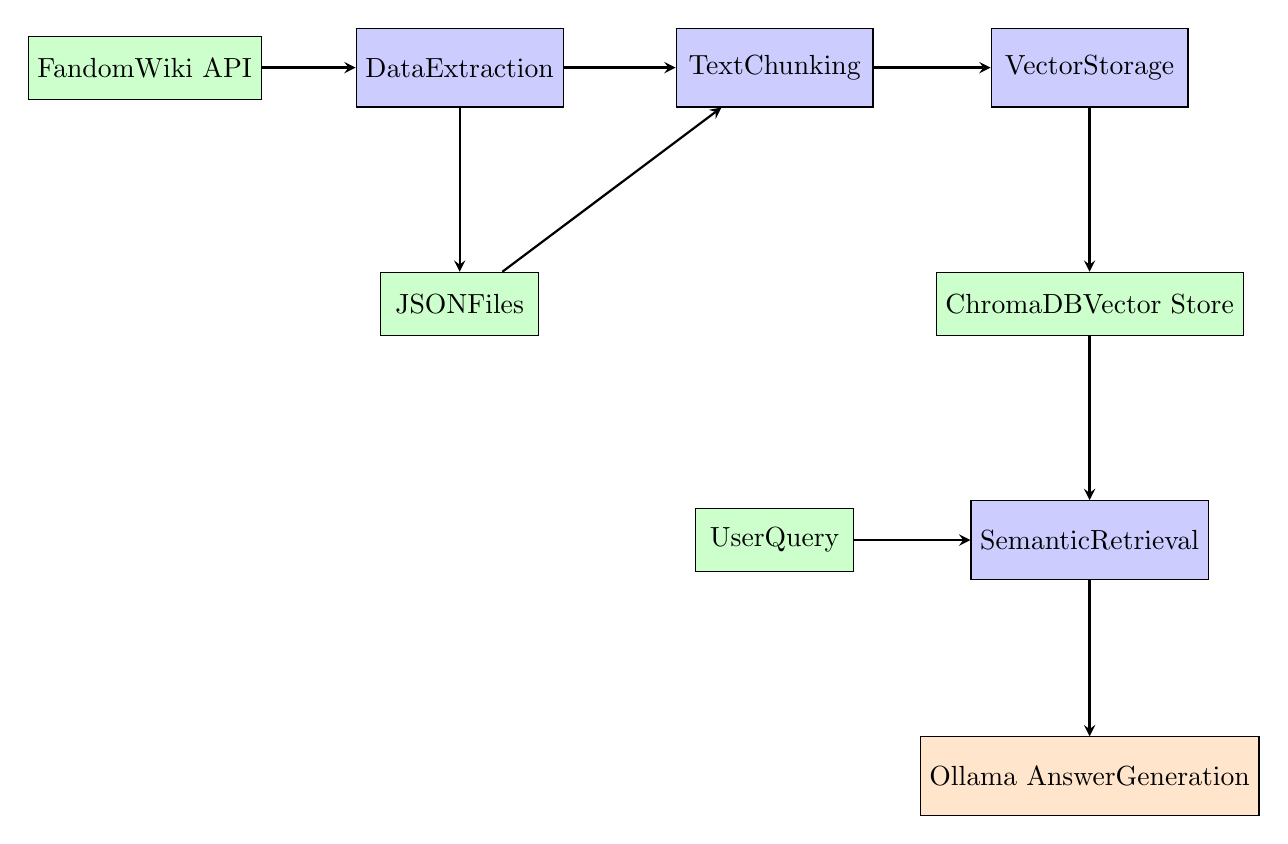
\begin{tikzpicture}[node distance=2cm, auto]
    % Define styles
    \tikzstyle{process} = [rectangle, minimum width=2.5cm, minimum height=1cm, text centered, draw=black, fill=blue!20]
    \tikzstyle{data} = [rectangle, minimum width=2cm, minimum height=0.8cm, text centered, draw=black, fill=green!20]
    \tikzstyle{llm} = [rectangle, minimum width=2.5cm, minimum height=1cm, text centered, draw=black, fill=orange!20]
    \tikzstyle{arrow} = [thick,->,>=stealth]
    
    % Nodes
    \node [data] (fandom) {Fandom\\Wiki API};
    \node [process, right of=fandom, xshift=2cm] (extract) {Data\\Extraction};
    \node [process, right of=extract, xshift=2cm] (chunk) {Text\\Chunking};
    \node [process, right of=chunk, xshift=2cm] (vectorize) {Vector\\Storage};
    \node [data, below of=extract, yshift=-1cm] (json) {JSON\\Files};
    \node [data, below of=vectorize, yshift=-1cm] (chromadb) {ChromaDB\\Vector Store};
    \node [process, below of=chromadb, yshift=-1cm] (retrieval) {Semantic\\Retrieval};
    \node [llm, below of=retrieval, yshift=-1cm] (llm_gen) {Ollama Answer\\Generation};
    \node [data, left of=retrieval, xshift=-2cm] (user) {User\\Query};
    
    % Arrows
    \draw [arrow] (fandom) -- (extract);
    \draw [arrow] (extract) -- (chunk);
    \draw [arrow] (chunk) -- (vectorize);
    \draw [arrow] (json) -- (chunk);
    \draw [arrow] (extract) -- (json);
    \draw [arrow] (vectorize) -- (chromadb);
    \draw [arrow] (chromadb) -- (retrieval);
    \draw [arrow] (retrieval) -- (llm_gen);
    \draw [arrow] (user) -- (retrieval);
    
\end{tikzpicture}
\caption{Book-Worm RAG System Architecture}
\label{fig:system_architecture}
\end{figure}

\subsection{Text Chunking Algorithm}

The chunking algorithm implements a section-based approach to optimize content for vector embeddings while preserving narrative coherence:

\begin{lstlisting}[language=Python, caption=Chunking Algorithm Implementation]
def merge_chunks_by_section(chunks, name, doc_type, series_name, max_words=400):
    # Group text by section headers
    section_map = defaultdict(list)
    for chunk in chunks:
        section_map[chunk['section']].append(chunk['text'])
    
    merged = []
    for section, paragraphs in section_map.items():
        # Combine all paragraphs in a section
        block = '\n\n'.join(paragraphs)
        words = block.split()
        
        # Split into fixed-size chunks of max_words
        for i in range(0, len(words), max_words):
            chunk_text = ' '.join(words[i:i+max_words])
            chunk_data = {
                'text': chunk_text,
                'section': section,
                'name': name,
                'type': doc_type,
                'series': series_name
            }
            merged.append(chunk_data)
    
    return merged
\end{lstlisting}

This algorithm:
\begin{itemize}
    \item Groups paragraphs by section headers to preserve context
    \item Splits text into fixed chunks of 400 words maximum
    \item Preserves metadata (section, name, type, series) for each chunk
    \item Ensures consistent chunk sizes for optimal vector embeddings
\end{itemize}

\section{Implementation}

\subsection{Technology Stack}

The implementation utilizes the following technologies:

\begin{itemize}
\item \textbf{Python 3.11}: Core implementation language
\item \textbf{ChromaDB}: Vector database for semantic search
\item \textbf{Requests}: HTTP client for API interactions
\item \textbf{Regular Expressions}: Text cleaning and parsing
\item \textbf{JSON}: Intermediate data storage format
\item \textbf{Ollama 3.2}: Answer generation through Ollama 3.2

\end{itemize}

\subsection{Series Configuration System}

The system employs a declarative configuration approach for adding new series:

\begin{lstlisting}[language=Python, caption=Series Configuration Example]
SERIES_CONFIG = {
    "Red Rising": {
        "wiki": "red-rising.fandom.com",
        "pages": [
            {"title": "Darrow_O'Lykos", 
             "type": "characters", 
             "name": "Darrow O'Lykos"},
            {"title": "Virginia_au_Augustus", 
             "type": "characters", 
             "name": "Mustang"},
            {"title": "The_Conquering", 
             "type": "events", 
             "name": "The Conquering"},
            {"title": "The_Institute", 
             "type": "locations", 
             "name": "The Institute"}
        ]
    },
    "Harry Potter": {
        "wiki": "harrypotter.fandom.com",
        "pages": [
            {"title": "Harry_Potter", 
             "type": "characters", 
             "name": "Harry Potter"},
            {"title": "Hermione_Granger", 
             "type": "characters", 
             "name": "Hermione Granger"}
        ]
    }
}
\end{lstlisting}

\section{Results}

The current implementation successfully processes multiple book series with the following metrics:

\begin{table}[H]
\centering
\begin{tabular}{lrrrr}
\toprule
\textbf{Series} & \textbf{Characters} & \textbf{Events} & \textbf{Locations} & \textbf{Total Chunks} \\
\midrule
Red Rising & 37 & 1 & 1 & 471 \\
Harry Potter & 3 & 0 & 0 & 382 \\
\midrule
\textbf{Total} & \textbf{40} & \textbf{1} & \textbf{1} & \textbf{853} \\
\bottomrule
\end{tabular}
\caption{Current System Processing Results}
\label{tab:processing_results}
\end{table}

\clearpage

\begin{figure}
    \centering
    \includegraphics[width=1\linewidth]{Screenshot 2025-11-28 at 8.29.33 PM.png}
    \caption{Character Query Results}
    \label{fig:placeholder}
\end{figure}

\clearpage

\begin{figure}
    \centering
    \includegraphics[width=1\linewidth]{Screenshot 2025-11-28 at 8.34.12 PM.png}
    \caption{Event Query Results}
    \label{fig:placeholder}
\end{figure}

\clearpage

\section{Future Work}

\begin{enumerate}
\item \textbf{Spoiler Tag}: Addition of spoiler tags for retrieved chunks with spoilers
\item \textbf{Additional Series}: New additions for any series requested for any user or myself
\end{enumerate}

\section{Conclusion}

This report showed the almost completed version of Book-Worm, a RAG system designed for multi-series books with guard rails for spoilers. Balancing spoiler limitations with proven to be difficult with the implementation of an LLM with guidelines, but have been getting consistent results for test queries for accurate retrievals and spoiler avoidance. Still need to perform further testing and add a spoiler tag for retried chunks to ensure correct answers are being retrieved while the strict spoiler filtering process occurs. Future work required is an the spoiler tag, and a potential for awareness for plot twists recognition, which may prove to be difficult. 

\pagebreak

\begin{thebibliography}{9}

\bibitem{angelidis2019bookqa}
Angelidis, S., Suhara, Y., Kannan, R., McAuley, J., \& Bansal, M. (2019). 
\textit{BookQA: Stories of Challenges and Opportunities}. 
In Proceedings of the 57th Annual Meeting of the Association for Computational Linguistics (pp. 693–703). 
Association for Computational Linguistics. Retrieved from https://aclanthology.org/P19-1067

\bibitem{mou2020frustratingly}
Mou, L., Wang, R., Li, G., Meng, L., \& Song, Y. (2020). 
\textit{Frustratingly Hard Evidence Retrieval for QA Over Books}. 
In Proceedings of the 2nd Workshop on Narrative Understanding (pp. 79–84). 
Association for Computational Linguistics. Retrieved from https://aclanthology.org/2020.nuse-1.13

\end{thebibliography}


\end{document}